% Versão em português brasileiro de main.tex.
% Mantenha este arquivo sincronizado com a versão em inglês: mesmas seções,
% tabelas, figuras, rótulos, citações e resultados. O abstract permanece em
% inglês; o resumo e o corpo do artigo estão em português.

\documentclass[12pt]{article}

\usepackage{sbc-template}
\usepackage{graphicx,url,booktabs}
\usepackage[utf8]{inputenc}
\usepackage[brazilian]{babel}

\sloppy

\title{Análise estatística e previsão da demanda por bicicletas compartilhadas:\\
um estudo observacional informado por DOE}

\author{[Primeiro autor]\inst{1}, [Segundo autor]\inst{1}}

\address{[Departamento e Universidade]\\
  Planejamento de Experimentos\\
  \email{[emails dos autores]}
}

\begin{document}

\maketitle

\begin{abstract}
This study analyses hourly bicycle rental demand using 17,379 observations from
the Capital Bikeshare system in Washington, D.C., collected in 2011 and 2012.
The data are observational and have a natural factorial and temporal structure.
We describe the response, examine the factors hour, working-day status, weather
situation and season through main-effect plots and the working-day by hour
interaction, and report a factorial analysis of variance. The raw count and its
logarithm are compared, and the logarithmic scale is adopted. A single
regression model with the working-day by hour interaction, weather situation,
season, temperature, humidity, wind speed and year is fitted, followed by basic
residual diagnostics. A strictly chronological split trains through September
2012 and tests on the last quarter of 2012. On the test set the model attains
MAE 45.27, RMSE 72.97 and $R^2$ 0.869. The associations are strong, but the
absence of randomisation prevents causal interpretation.
\end{abstract}

\begin{resumo}
Este estudo analisa a demanda horária por bicicletas usando 17.379 observações
do sistema Capital Bikeshare de Washington, D.C., coletadas em 2011 e 2012. Os
dados são observacionais e possuem estrutura fatorial e temporal natural.
Descrevemos a resposta, examinamos os fatores hora, tipo de dia, situação
climática e estação por meio de gráficos de efeitos principais e da interação
entre tipo de dia e hora, e apresentamos uma análise de variância fatorial. A
contagem bruta e seu logaritmo são comparados, adotando-se a escala logarítmica.
Um único modelo de regressão com a interação tipo de dia por hora, situação
climática, estação, temperatura, umidade, velocidade do vento e ano é ajustado,
seguido de diagnósticos básicos dos resíduos. Uma divisão estritamente temporal
treina até setembro de 2012 e testa no último trimestre de 2012. No conjunto de
teste, o modelo atinge MAE 45,27, RMSE 72,97 e $R^2$ 0,869. As associações são
fortes, mas a ausência de randomização impede interpretação causal.
\end{resumo}

\section{Introdução}

Sistemas de compartilhamento de bicicletas registram demanda com alta resolução
temporal e oferecem uma visão útil da mobilidade urbana. O número de aluguéis
depende simultaneamente de condições de calendário, sazonais e meteorológicas.
Essa estrutura multifatorial torna os dados adequados a uma perspectiva de
Planejamento de Experimentos (DOE), embora os registros não tenham sido
produzidos por um experimento controlado.

O objetivo é identificar e quantificar os fatores associados à demanda horária
por aluguéis e avaliar a predição em um período posterior. Atenção especial é
dada à interação entre hora e tipo de dia: deslocamentos devem gerar picos
matinais e vespertinos em dias úteis, enquanto dias não úteis devem apresentar
perfil recreativo mais suave. Como nenhum tratamento foi randomizado, a análise
usa linguagem de associação e predição em todo o texto.

\section{Base de dados e desenho do estudo}

A base UCI Bike Sharing Dataset \cite{uci-bike-sharing} contém registros do
sistema Capital Bikeshare em Washington, D.C.; a publicação associada descreve a
coleta dos dados \cite{fanaee2013}. Usamos o arquivo horário, que cobre de 1 de
janeiro de 2011 a 31 de dezembro de 2012. Cada linha corresponde a uma hora
observada.

A resposta, \texttt{cnt}, é o total de aluguéis e equivale a
\texttt{casual + registered}. Ambos os componentes são excluídos como
preditores porque causariam vazamento da resposta. Os quatro fatores são hora
(\texttt{hr}), tipo de dia (\texttt{workingday}), situação climática
(\texttt{weathersit}) e estação (\texttt{season}). Temperatura, umidade e
velocidade do vento são covariáveis contínuas padronizadas. A temperatura
aparente não é usada porque sua correlação com a temperatura é $0{,}988$.

O desenho é observacional, não randomizado, sem blocos e naturalmente fatorial;
não é um experimento controlado. As observações são ordenadas no tempo e não
podem ser consideradas independentes. Há 165 horários ausentes no calendário
horário, e não foi feita imputação. O nível 4 da situação climática ocorre em
apenas três horas, de modo que sua estimativa descritiva é necessariamente
imprecisa.

\section{Métodos}

\subsection{Análise descritiva e gráficos fatoriais}

Calculamos tamanhos amostrais, médias, medianas, desvios-padrão, quartis,
histogramas, boxplots, uma série temporal diária e correlações de Pearson para
\texttt{cnt}. Os gráficos de efeitos principais mostram a média de cada nível
dos quatro fatores com intervalos de confiança de 95\%. Um segundo gráfico mostra
a demanda média por hora separadamente para dias úteis e não úteis, tornando
visível a interação entre hora e tipo de dia.

\subsection{Análise de variância fatorial}

Um modelo fatorial foi ajustado por mínimos quadrados ordinários com os quatro
fatores, as três covariáveis contínuas e o ano como ajustes, além da interação
entre hora e tipo de dia. Uma análise de variância tipo II reporta o eta
quadrado parcial de cada termo \cite{montgomery2017}. Como o desenho é
observacional e desbalanceado, a magnitude dos efeitos e a validação temporal
são enfatizadas em vez da significância isoladamente.

\subsection{Escala da resposta}

A resposta bruta \texttt{cnt} e $\log(1+\texttt{cnt})$ foram comparadas na mesma
estrutura de modelo usando gráficos de resíduos versus ajustados, gráficos
normais Q--Q, o teste de Shapiro--Wilk em subconjunto fixo de 5.000 resíduos e o
teste studentizado de Breusch--Pagan para variância constante. A função de
autocorrelação (ACF) dos resíduos também foi examinada. A escala logarítmica foi
adotada porque melhorou o ajuste e reduziu a estatística de Breusch--Pagan; isso
não implica que a pressuposição de normalidade seja satisfeita.

\subsection{Regressão e diagnósticos dos resíduos}

Um único modelo de regressão foi especificado antes do ajuste:
\begin{center}
\texttt{log1p(cnt) $\sim$ C(hr) * C(workingday) + C(weathersit) + C(season)} \\
\texttt{$\quad$ + temp + hum + windspeed + C(yr).}
\end{center}
A interação inclui ambos os efeitos principais componentes. Os diagnósticos
básicos consistem em gráficos de resíduos versus ajustados, gráficos normais
Q--Q e da ACF dos resíduos em defasagens de horas observadas. A correção de
smearing de Duan foi usada para transformar as previsões de volta à escala de
contagem \cite{duan1983}.

\subsection{Divisão temporal entre treino e teste}

O modelo foi treinado em todas as horas até 30 de setembro de 2012 e avaliado nas
2.168 horas de 1 de outubro a 31 de dezembro de 2012. A divisão é estritamente
temporal e mantém os dois anos nos dados de treino, de modo que o fator ano é
estimável. A divisão aleatória foi evitada porque misturaria observações futuras
e passadas. O desempenho no teste é reportado com erro absoluto médio (MAE),
raiz do erro quadrático médio (RMSE) e $R^2$ fora da amostra na escala de
contagem.

\section{Resultados}

\subsection{Resultados descritivos}

A Tabela~\ref{tab:descriptive} resume a resposta. A média excede a mediana e a
distribuição bruta é assimétrica à direita (assimetria $1{,}277$).

\begin{table}[ht]
\centering
\caption{Estatísticas descritivas dos aluguéis horários totais.}
\label{tab:descriptive}
\resizebox{\columnwidth}{!}{\begin{tabular}{rrrrrrrr}
\toprule
N & Mean & Median & SD & Q1 & Q3 & Min & Max \\
\midrule
17379 & 189.463 & 142.000 & 181.388 & 40.000 & 281.000 & 1.000 & 977.000 \\
\bottomrule
\end{tabular}
}
\end{table}

A demanda horária média foi $204{,}87$ com tempo claro ou parcialmente nublado,
$175{,}17$ com névoa ou nublado, $111{,}58$ com precipitação leve e $74{,}33$ com
tempo severo, este último com apenas três horas. As médias sazonais foram
$111{,}11$ na primavera, $208{,}34$ no verão, $236{,}02$ no outono e $198{,}87$
no inverno. Essas associações não ajustadas refletem desequilíbrios entre as
demais condições.

\begin{figure}[ht]
\centering
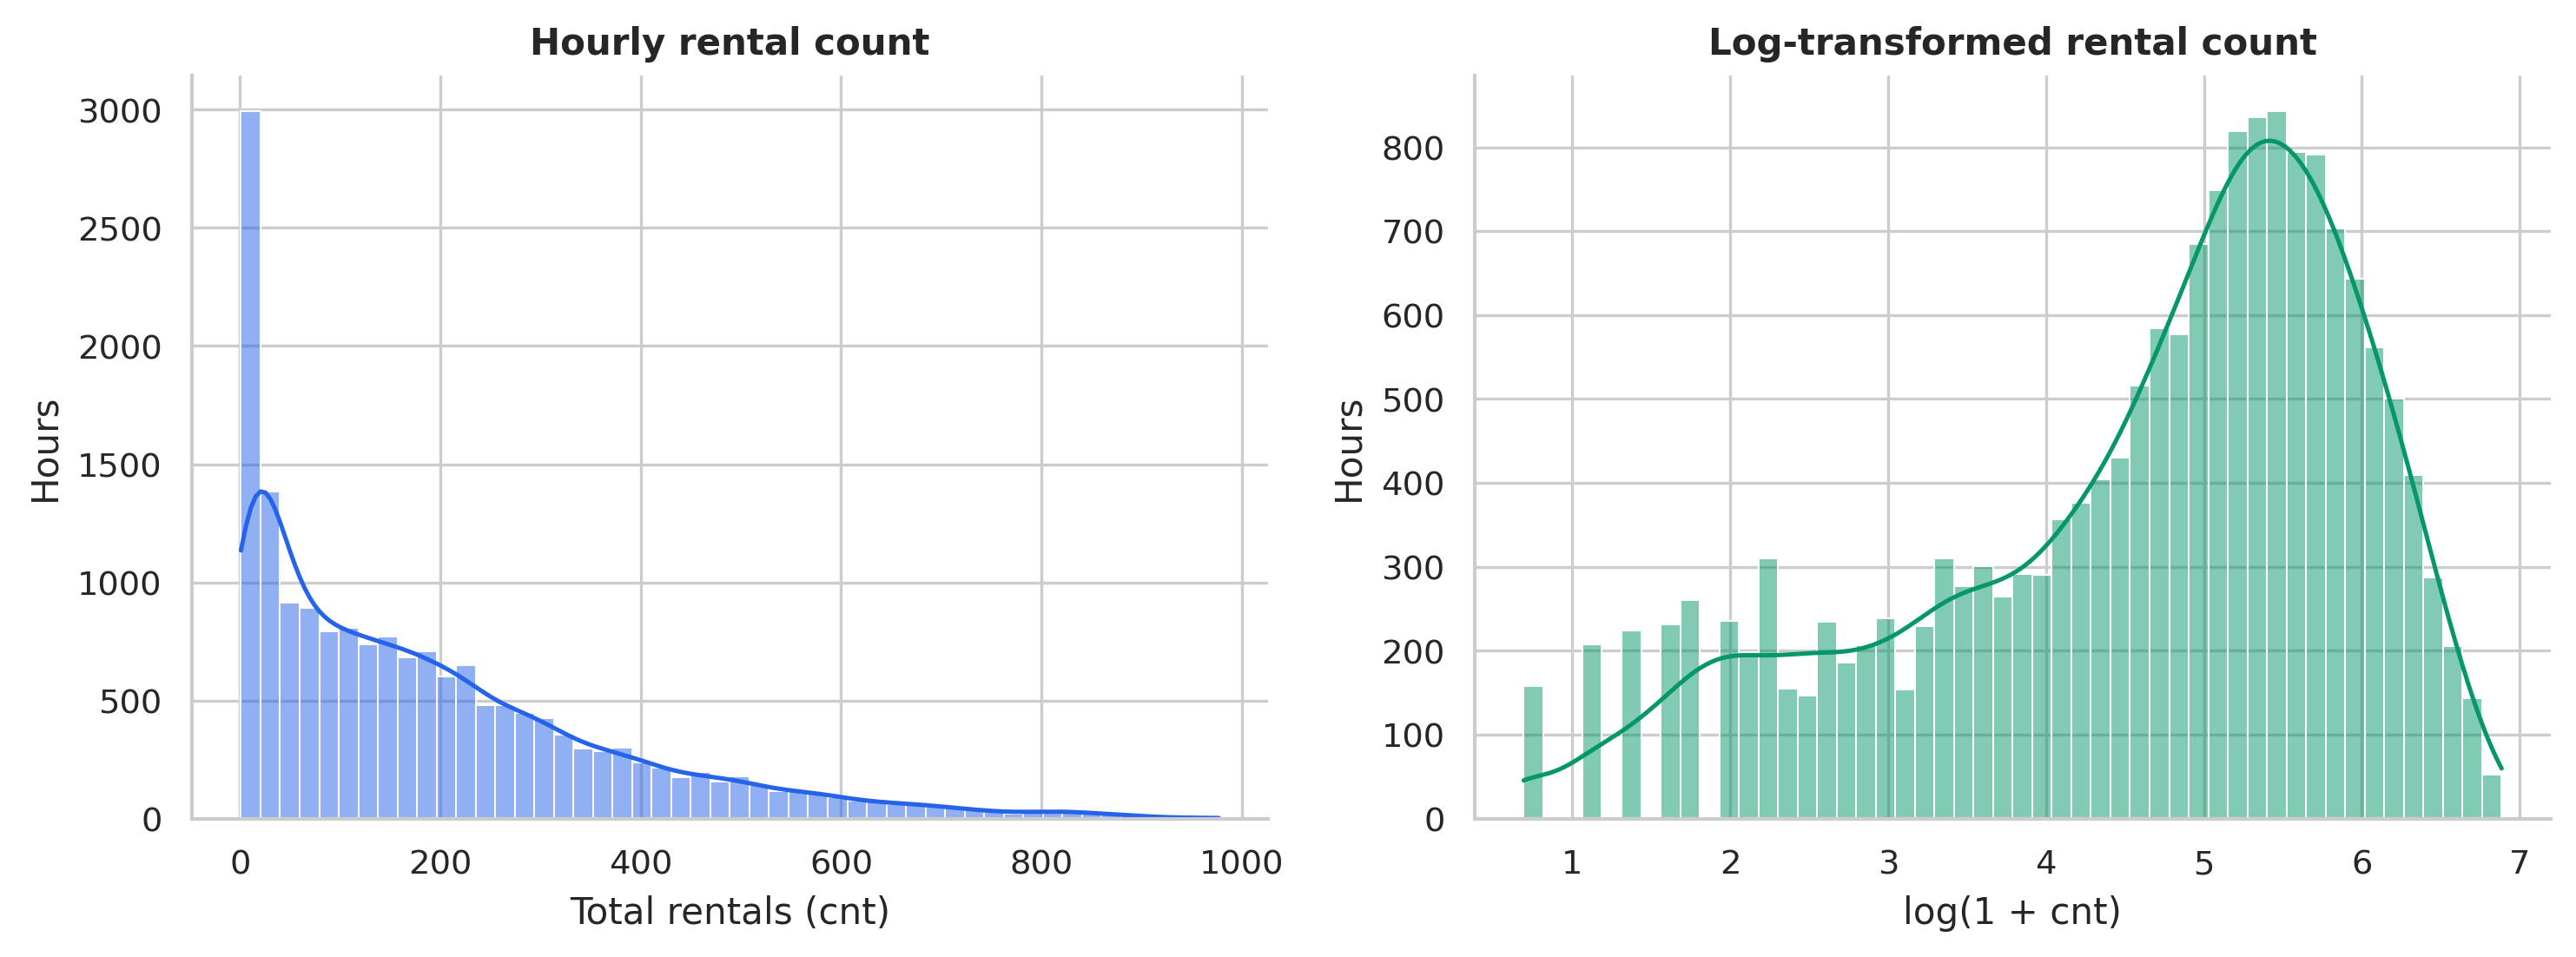
\includegraphics[width=\columnwidth]{../outputs/figures/response_distributions.png}
\caption{Distribuições dos aluguéis horários nas escalas bruta e log-transformada.}
\label{fig:distribution}
\end{figure}

\subsection{Efeitos principais e interação}

A Figura~\ref{fig:main-effects} mostra os quatro efeitos principais. Hora e
estação são as margens mais visíveis; o tipo de dia apresenta pequena diferença
média incondicional. A Figura~\ref{fig:workingday-hour} mostra por que essa
diferença não deve ser lida isoladamente: em dias úteis a demanda atinge pico
por volta das 08:00 e entre 17:00--18:00, enquanto dias não úteis apresentam pico
mais amplo ao meio do dia.

\begin{figure}[ht]
\centering
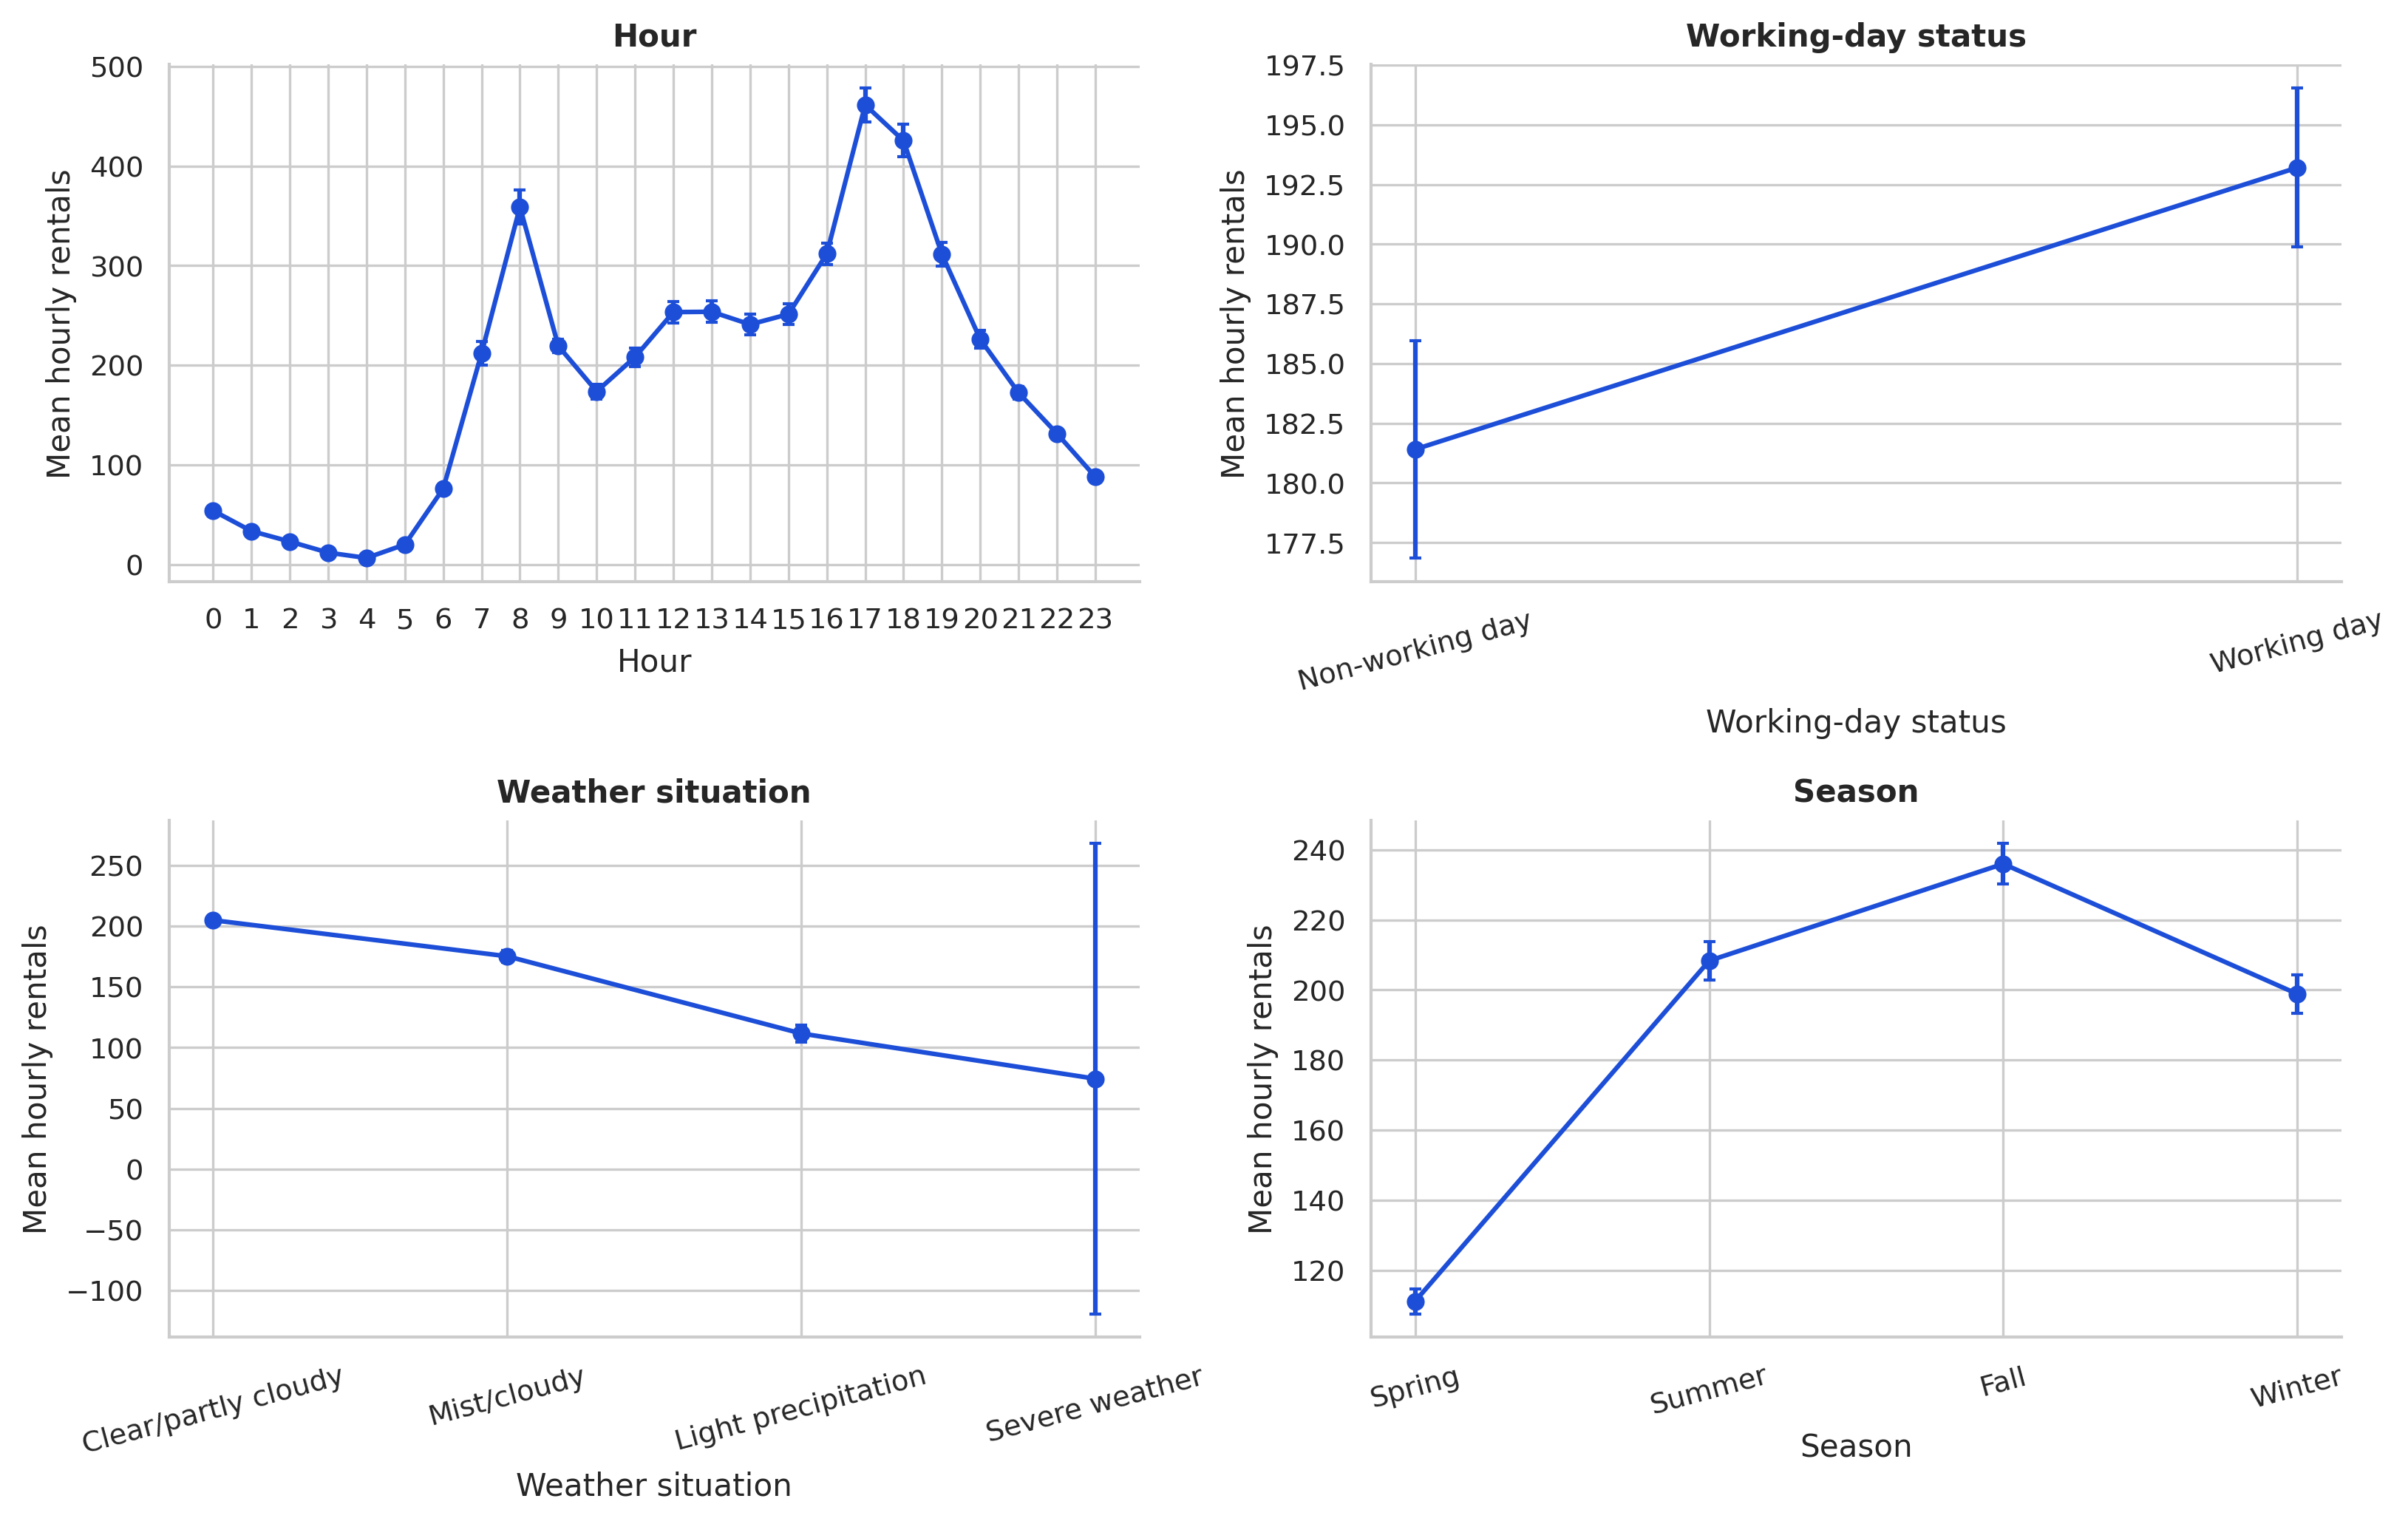
\includegraphics[width=\columnwidth]{../outputs/figures/main_effects.png}
\caption{Gráficos de efeitos principais para hora, tipo de dia, situação climática e estação.}
\label{fig:main-effects}
\end{figure}

\begin{figure}[ht]
\centering
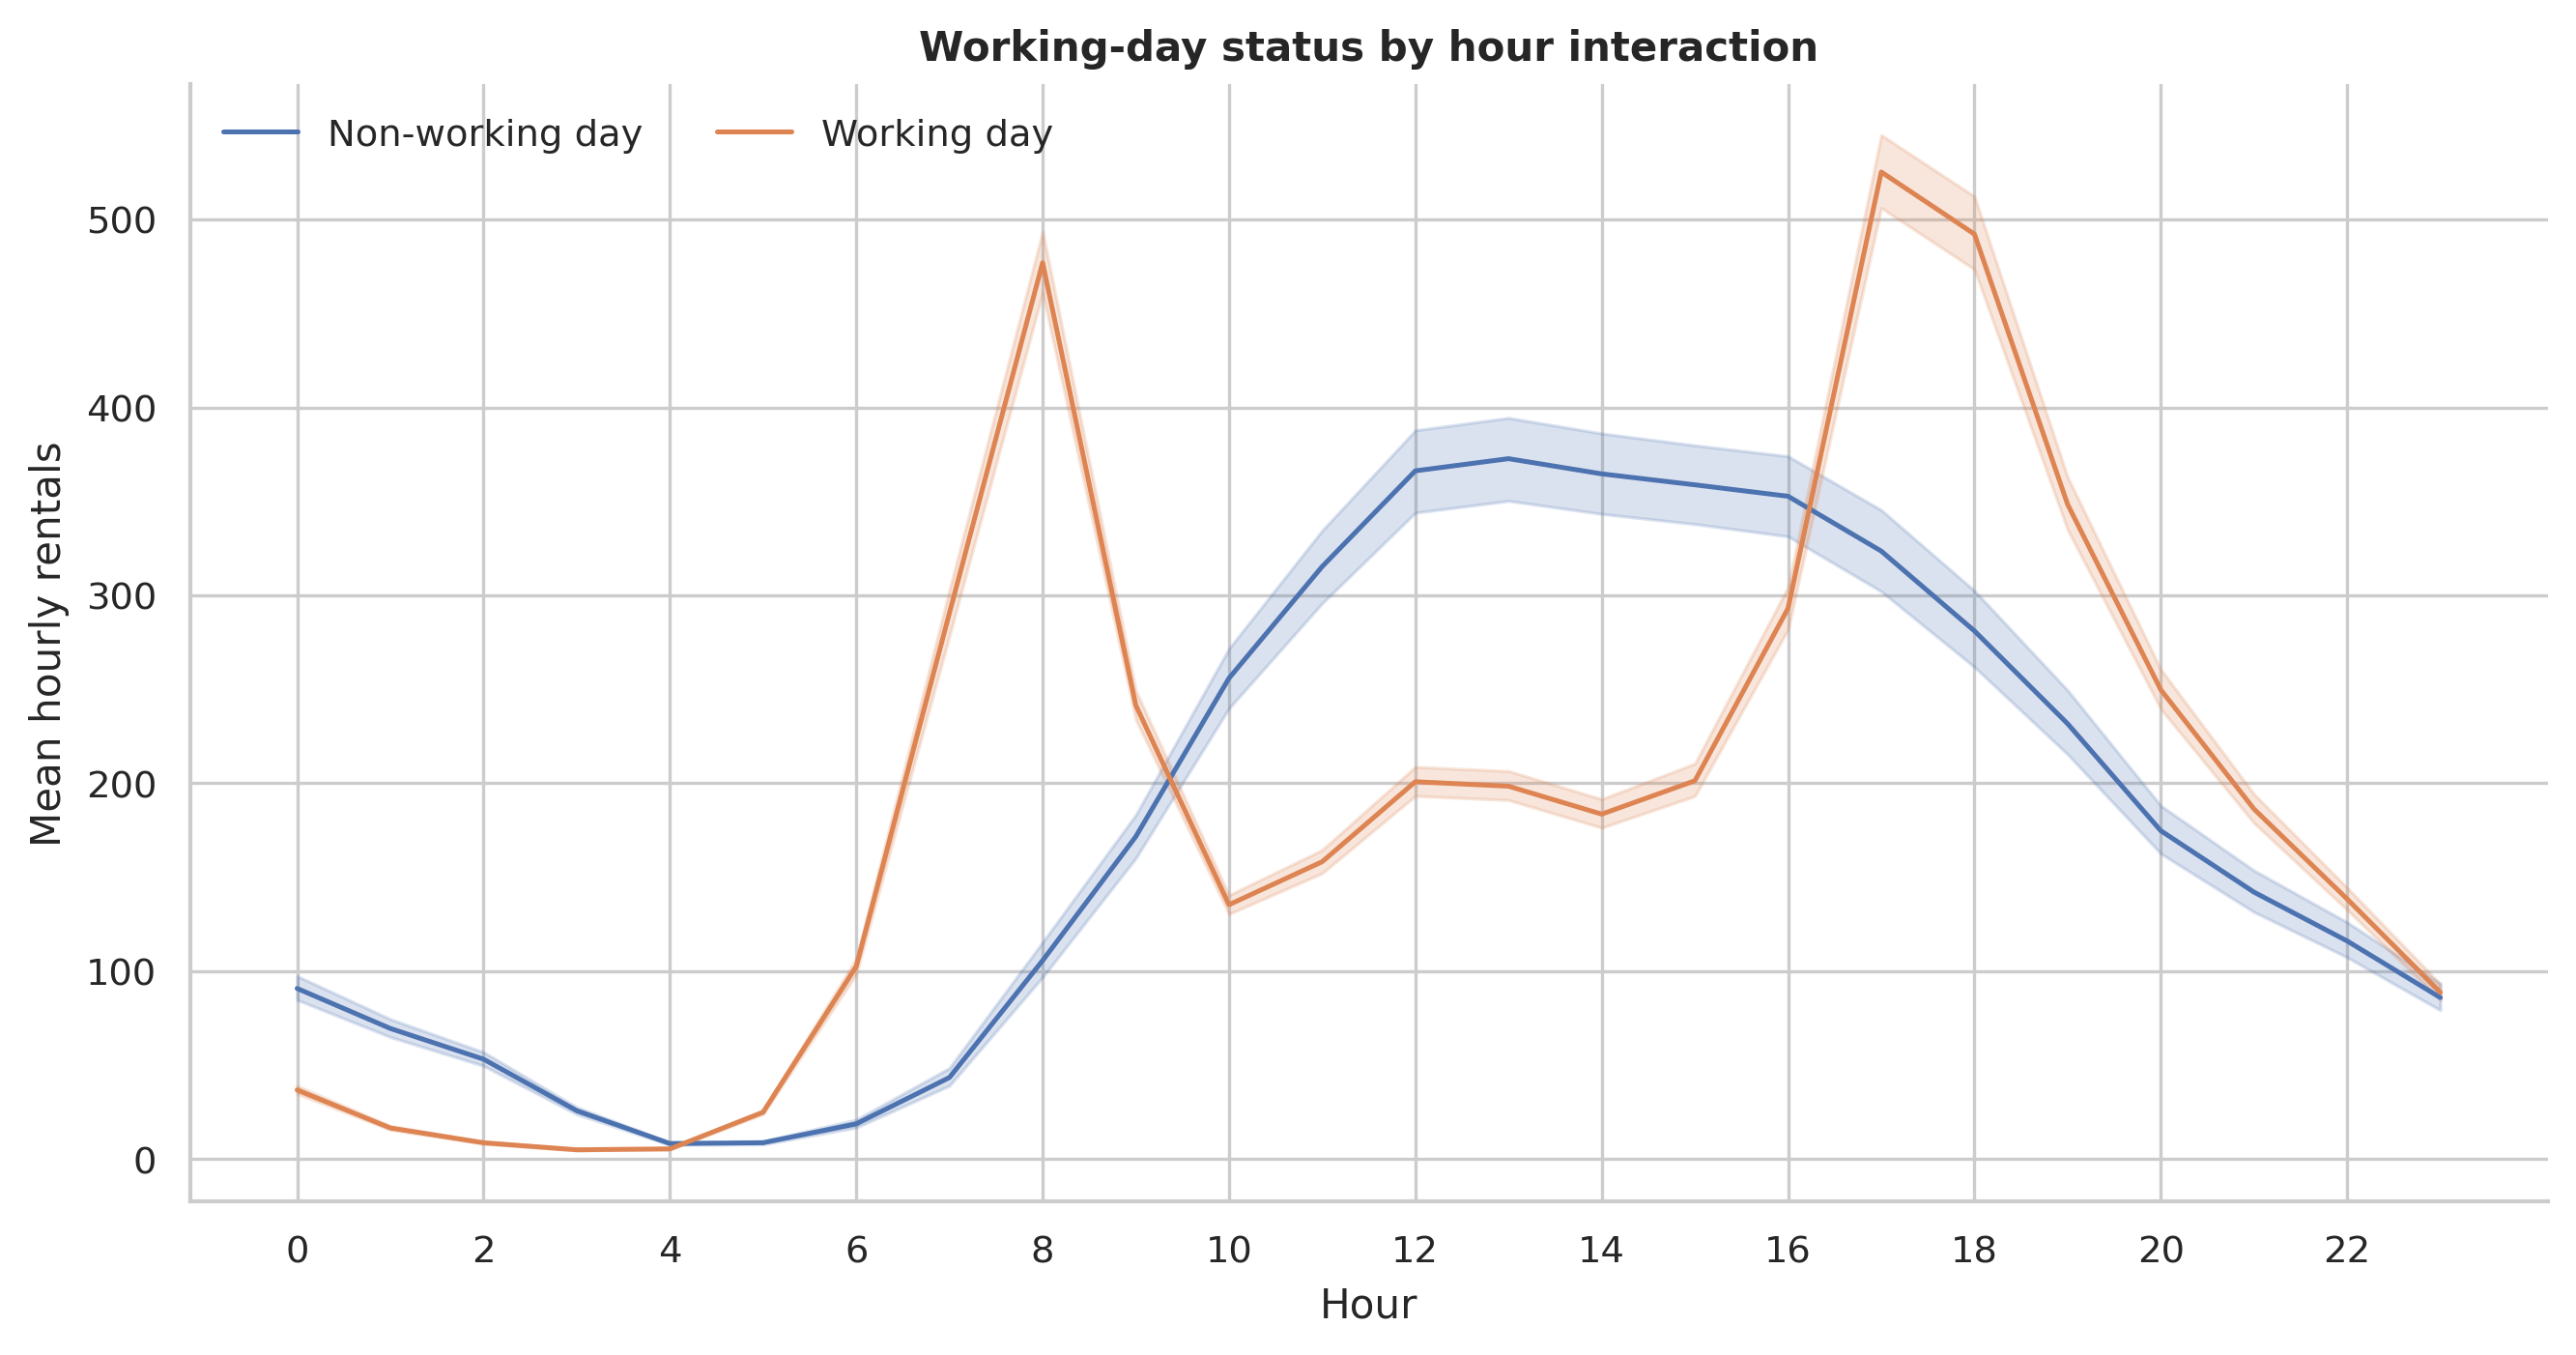
\includegraphics[width=\columnwidth]{../outputs/figures/workingday_hr_interaction.png}
\caption{Interação entre tipo de dia e hora.}
\label{fig:workingday-hour}
\end{figure}

\subsection{ANOVA fatorial}

A Tabela~\ref{tab:anova} apresenta a ANOVA fatorial tipo II. A hora possui eta
quadrado parcial $0{,}878$ e a interação hora por tipo de dia, $0{,}589$. A
situação climática e a estação contribuem com $0{,}120$ e $0{,}168$,
respectivamente, e o ano com $0{,}264$. O efeito principal de tipo de dia é
pequeno ($0{,}001$), coerente com o gráfico de interação.

\begin{table}[ht]
\centering
\caption{ANOVA fatorial tipo II para o modelo na escala logarítmica.}
\label{tab:anova}
\resizebox{\columnwidth}{!}{\begin{tabular}{lrrlr}
\toprule
Term & df & F & p-value & Partial eta-squared \\
\midrule
Hour & 23.000 & 6050.916 & $<0.001$ & 0.890 \\
Working day & 1.000 & 19.488 & $<0.001$ & 0.001 \\
Weather & 2.000 & 1283.947 & $<0.001$ & 0.130 \\
Season & 3.000 & 820.348 & $<0.001$ & 0.125 \\
Year & 1.000 & 6367.468 & $<0.001$ & 0.270 \\
Hour x working day & 23.000 & 1195.618 & $<0.001$ & 0.615 \\
Weather x hour & 46.000 & 7.820 & $<0.001$ & 0.020 \\
Season x hour & 69.000 & 8.444 & $<0.001$ & 0.033 \\
Temperature & 1.000 & 2253.208 & $<0.001$ & 0.116 \\
Temperature squared & 1.000 & 1020.639 & $<0.001$ & 0.056 \\
Humidity & 1.000 & 287.999 & $<0.001$ & 0.016 \\
Wind speed & 1.000 & 198.396 & $<0.001$ & 0.011 \\
\bottomrule
\end{tabular}
}
\end{table}

\subsection{Escala da resposta e diagnósticos dos resíduos}

A Tabela~\ref{tab:scales} compara as duas escalas. O $R^2$ ajustado sobe de
$0{,}812$ em \texttt{cnt} para $0{,}927$ em $\log(1+\texttt{cnt})$, enquanto a
estatística de Breusch--Pagan cai de $4281{,}6$ para $1676{,}6$. Shapiro--Wilk
rejeita normalidade nas duas escalas, de modo que a escolha do log se baseia em
variância e ajuste, não em uma afirmação de resíduos normais. O modelo ajustado
usa 58 parâmetros, com AIC $15916{,}2$ e BIC $16366{,}4$.

\begin{table}[ht]
\centering
\caption{Comparação entre as escalas bruta e logarítmica da resposta.}
\label{tab:scales}
\resizebox{\columnwidth}{!}{\begin{tabular}{lrrr}
\toprule
Response & Adjusted $R^2$ & Shapiro--Wilk $W$ ($p$) & Breusch--Pagan LM ($p$) \\
\midrule
$cnt$ & 0.812 & 0.972 ($<0.001$) & 4282.8 ($<0.001$) \\
$\log(1+cnt)$ & 0.927 & 0.949 ($<0.001$) & 1672.5 ($<0.001$) \\
\bottomrule
\end{tabular}
}
\end{table}

A ACF dos resíduos é $0{,}612$ na defasagem 1, $0{,}243$ na defasagem 24 e
$0{,}200$ na defasagem 168 (Figura~\ref{fig:acf}), mostrando dependência temporal
não explicada pelos fatores incluídos. Consequentemente, a significância
reportada é descritiva e o conjunto de teste temporal é a principal evidência
de desempenho preditivo.

\begin{figure}[ht]
\centering
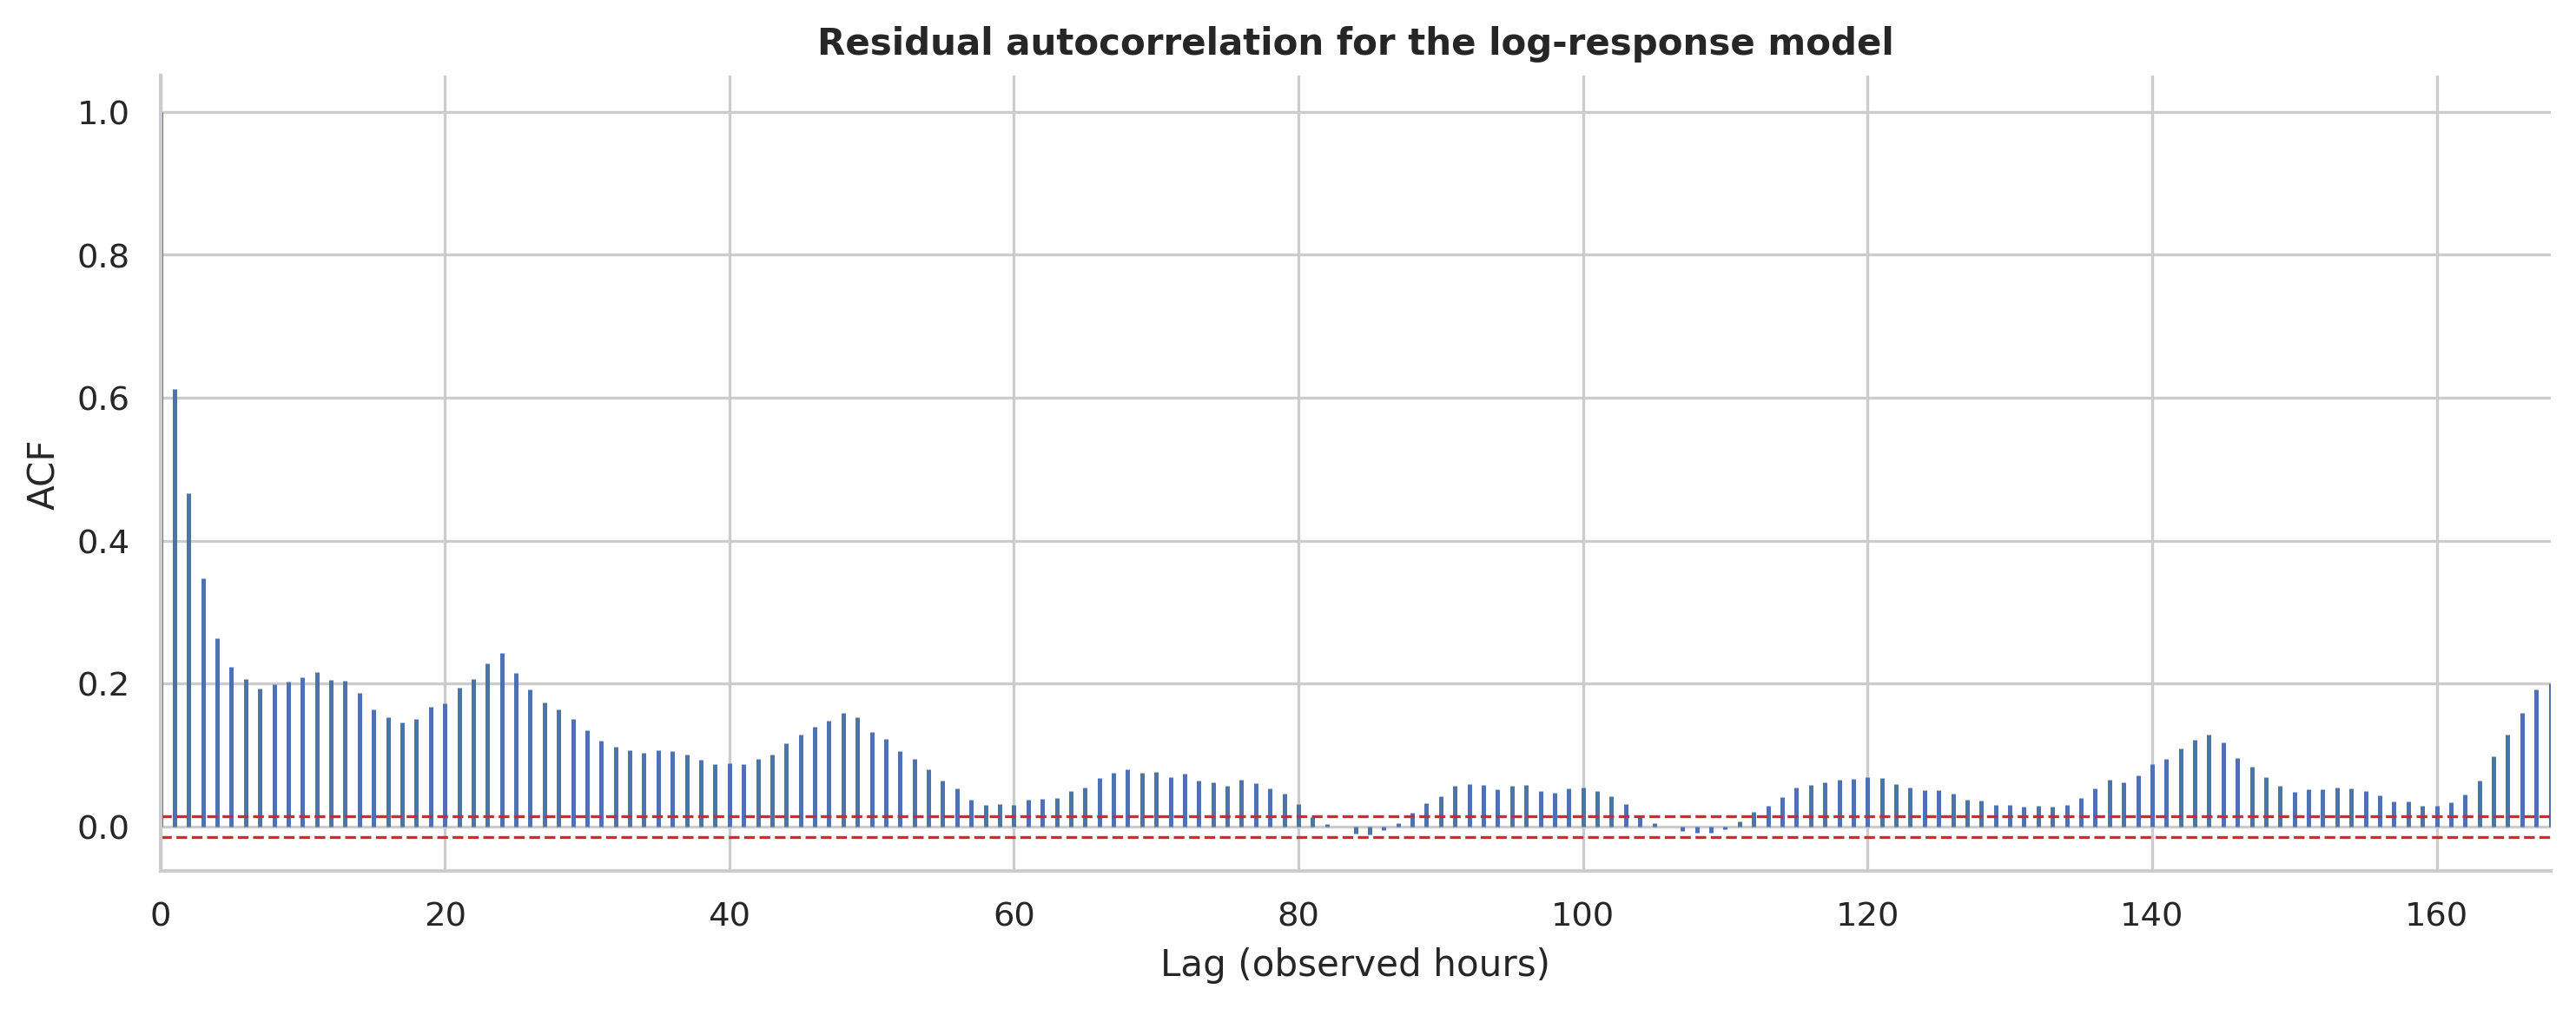
\includegraphics[width=\columnwidth]{../outputs/diagnostics/residual_acf.png}
\caption{Função de autocorrelação dos resíduos do modelo na escala logarítmica.}
\label{fig:acf}
\end{figure}

\subsection{Desempenho no conjunto de teste}

Nas 2.168 horas de teste, o modelo obteve MAE $45{,}27$, RMSE $72{,}97$ e
$R^2=0{,}869$ (Tabela~\ref{tab:test} e Figura~\ref{fig:predictions}). O período
de teste é um trimestre de outono, de modo que o resultado descreve uma
extrapolação de curto prazo dentro do sistema observado em dois anos.

\begin{table}[ht]
\centering
\caption{MAE, RMSE e $R^2$ no conjunto de teste do Q4/2012.}
\label{tab:test}
\resizebox{\columnwidth}{!}{\begin{tabular}{rrr}
\toprule
MAE & RMSE & Test $R^2$ \\
\midrule
45.267 & 72.966 & 0.869 \\
\bottomrule
\end{tabular}
}
\end{table}

\begin{figure}[ht]
\centering
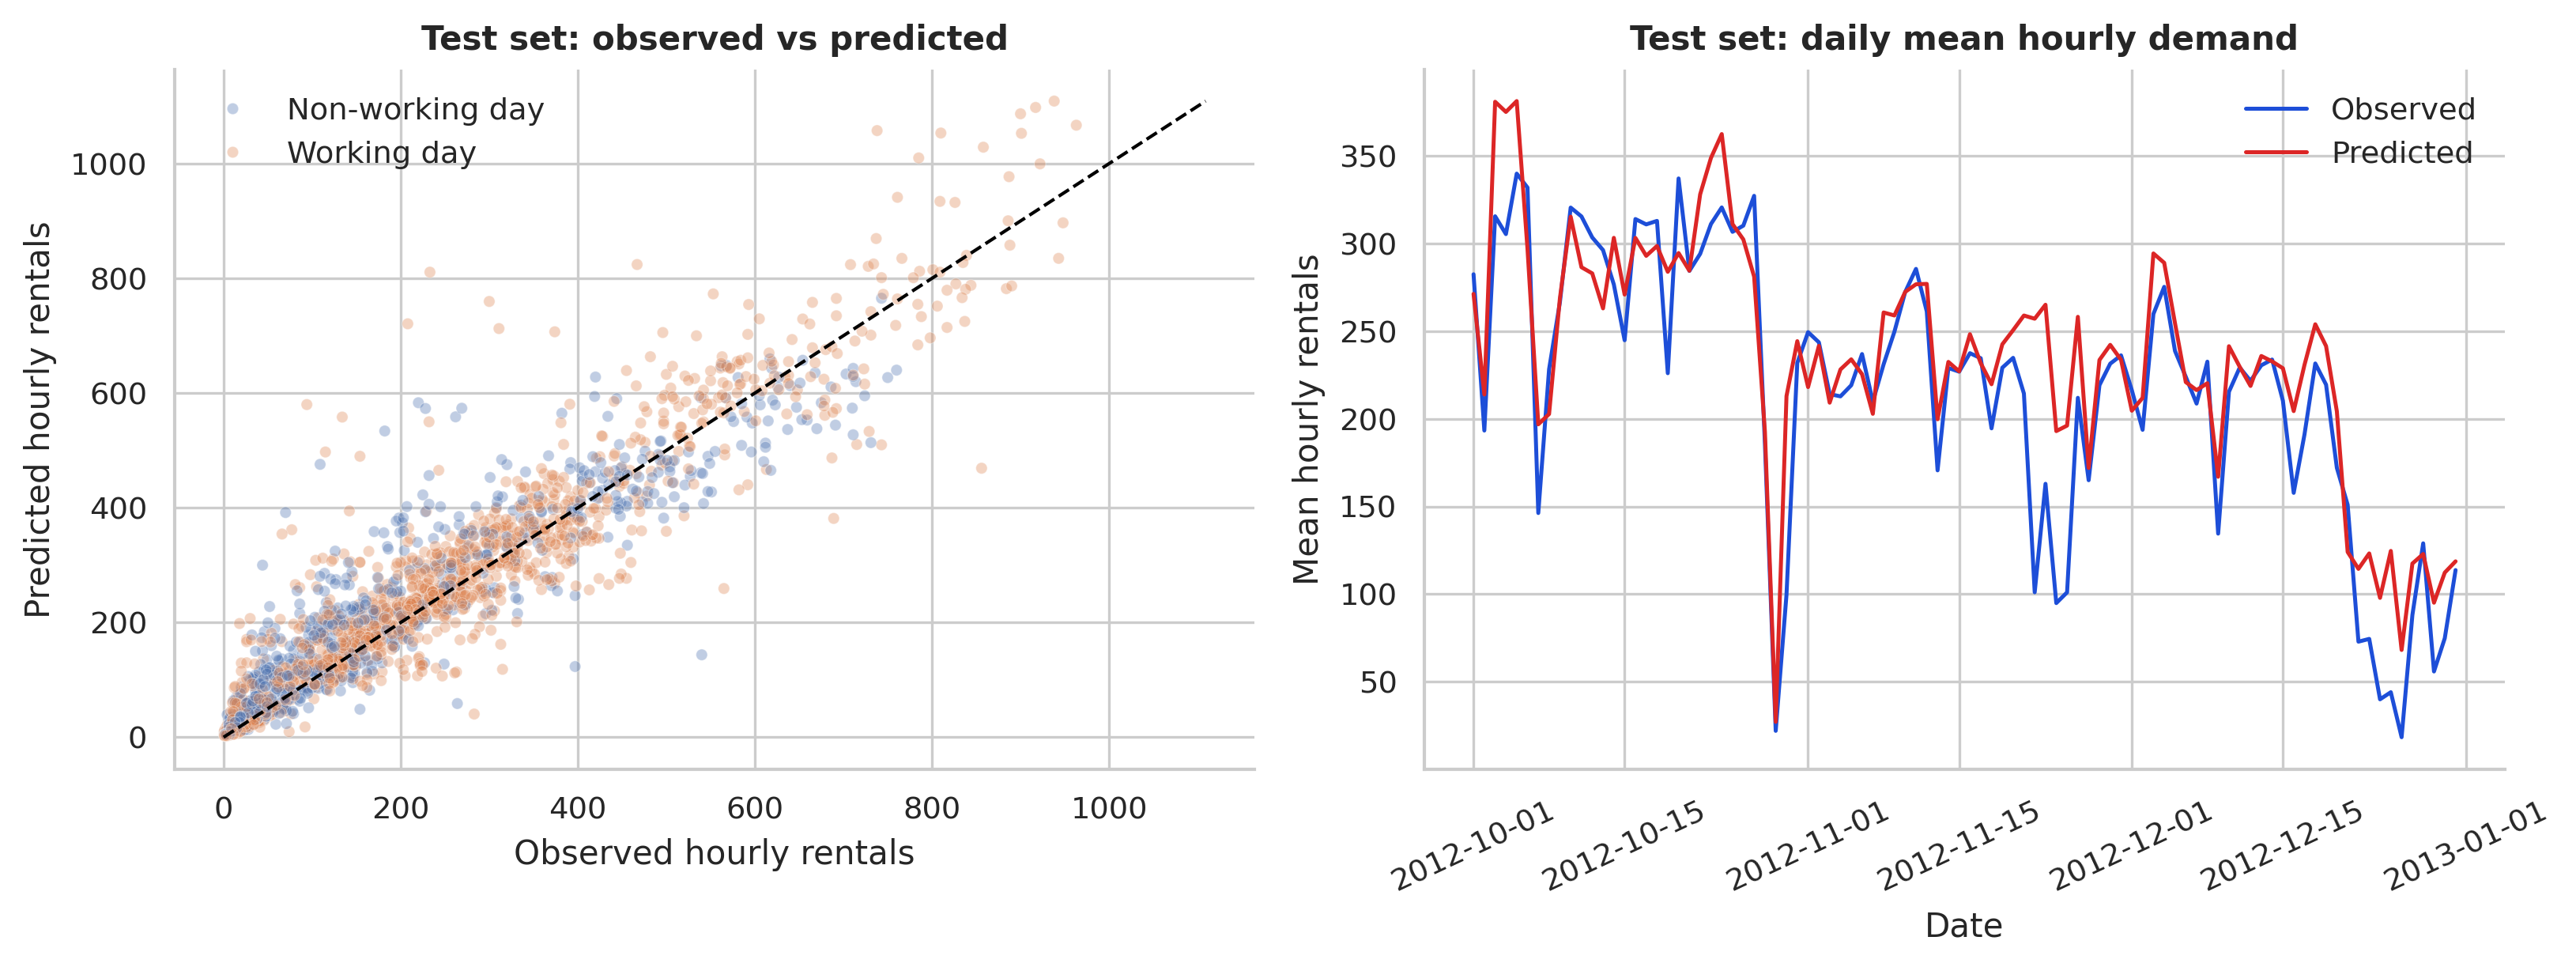
\includegraphics[width=\columnwidth]{../outputs/figures/test_predictions.png}
\caption{Demanda observada e prevista no conjunto de teste.}
\label{fig:predictions}
\end{figure}

\section{Discussão e limitações}

A hora é o fator dominante, mas sua forma depende fortemente do tipo de dia, que
é exatamente o que a análise fatorial permite revelar. Situação climática,
estação, temperatura e ano fornecem ajuste relevante. A análise é limitada pela
ausência de randomização: eventos não medidos, expansão do sistema e tendências
temporais podem confundir as estimativas. A autocorrelação residual permanece
após os fatores incluídos, e três horas com tempo severo não permitem uma
estimativa separada precisa. Modelos de efeitos mistos, autoregressivos e de
distribuição de contagem não foram investigados.

\section{Conclusão}

A análise identifica a interação entre tipo de dia e hora como a principal
característica estrutural da demanda horária por bicicletas, com eta quadrado
parcial $0{,}589$. O único modelo de regressão em $\log(1+\texttt{cnt})$ atinge
$R^2$ ajustado $0{,}927$ e prevê um trimestre não visto com $R^2=0{,}869$,
MAE $45{,}27$ e RMSE $72{,}97$. Os resultados sustentam uso descritivo e
preditivo, não inferência causal.

\bibliographystyle{sbc}
\bibliography{references}

\end{document}
